\documentclass[11pt]{article}
\usepackage{graphicx}
\usepackage{geometry}

\geometry{
	left=25mm,
	right=25mm,
	top=25mm,
	bottom=25mm,
}
\begin{document}
	
	\begin{center}
		\textbf{ASSIGNMENT– 5}
	\end{center}
	\textbf{AIM:}
	Implement Decision trees on Digital Library Data to mirror moretitles (PDF) in the library application, compare it with Nave Bayes algorithm. \\ 
	
	\noindent \textbf{OBJECTIVE:}
	\begin{itemize}
		\item To understand the basic concept to K-means Clustering.
		\item To implement K-means clustering algorithm using Java.
	\end{itemize}
	
	\noindent \textbf{SOFTWARE REQUIREMENTS:}
	\begin{itemize}
		\item Linux Operating System
		\item Java compiler
		\item Weka Tool
	\end{itemize}•
	
	\noindent \textbf{MATHEMATICAL MODEL:} \\
	Consider a set S consisting of all the elements related to a program. \\
	The Mathematical model is given as below, \\
	S={s,e,X,Y,Fme,DD,NDD,Mem shared} \\
	Where, \\
	s=Initial State \\
	e=End State \\
	X=Input. Here it is number of elements, actual element, number of clusters \\
	Y=Output. Here output isfn al cluster by K-means. \\
	Fme=Algorithm/Functionusedinprogram.foreg.fcalmean(),caldif()g
	DD=Deterministic Data \\
	NDD=NondeterministicData \\
	Memshared=Memorysharedbyprocessor. \\
	
	\noindent \textbf{THEORY:} \\
	
	\textbf{DecisionTree:} \\
	\paragraph{}
	Adecisiontreeis adecision supporttool that uses a tree-likegraph ormodel
	ofdecisionsand theirpossible consequences,includingchanceevent outcomes, resource
	costs,andutility.It is onewayto displayanalgorithm.
	Decisiontreesare commonlyusedinoperationsresearch, specificallyindecision analysis, tohelp
	identifyastrategymost likelytoreach agoal. \\
	
	\textbf{K-meansClustering:} \\
	\paragraph{}
	k-means is one of the simplest unsupervised learning algorithms that
	solve the well known clustering problem. The procedure follows asimple and easy wayto
	classify a given data set through a certain number of clusters(assume kclusters)fxed apriori. The
	main idea is to defne k center, one for each ncluster. These centers should be placed in a cunning
	way because of diferent location causes different result. So, the better choice is to place them as
	much as possible far away from eachother. The next step is to take each point belong in gto
	agiven data set and as satiate it to the nearest center. When no point is pending, the frst step is
	completed and an early group age is done. At this point we need to re-calculate k new centroids
	as barycenterof the clusters resulting from the previous step. After we have these k new
	centroids, a new binding has to bedone between the same data set points and the nearest new
	center. A loop has been generated. As a result of this loop we may notice that the k centers
	change their location step by step until no more changes are done or in other words centers do
	not move anymore. Finally, this algorithm aims at minimizing
	an objective function know as squared error function given by:
	J(V)=(xi-vj)2 (1)
	Where,
	xi-vjisthe Euclidean distance betweenxi and vj.
	`ci’ is the number of data points in ith cluster.
	`c’ is the number of cluster centers. \\
	
	\textbf{Algorithmic steps fork-means clustering:} \\
	\paragraph{}
	
	Let X=fx1,x2,x3,..,xngbethe set of data points andV =fv1,v2,.,vcgbethe
	set of centers.
	\begin{enumerate}
		\item Randomly select `c’ cluster centers.
		\item Calculate the distance between each data point and cluster centers.
		\item Assign the data point to the cluster center whose distance from the cluster center is
		minimumof all the cluster centers.
		\item Recalculate the new cluster center using: Vi = (1=Ci)Xi (2)
		where, `ci’ represents the number of data points in ith cluster.
		\item Recalculate the distance between each data point and new obtained cluster centers.
		\item If no data point was reassigned then stop, otherwise repeat from step 3.
		
	\end{enumerate}
	
	\noindent \textbf{Advantages:} \\
	\begin{enumerate}
		\item Fast, robust and easier to understand.
		\item Relatively efcient: O(tknd), where n is objects, k is  clusters, d is  dimension of each
		object, and t is  iterations. Normally,k, t, d <<n.
		\item Gives best result when dataset are distinct or well separated from each other.
	\end{enumerate}•
	
	
	\noindent \textbf{Disadvantages:} \\
	\begin{enumerate}
		\item The learning algorithm requires apriori specifcation ofthe number of cluster centers.
		\item The use of Exclusive Assignment-If there are two highly overlapping data then k-means
		willnot be
		able to resolve that there aretwo clusters.
		\item Thelearning algorithm is not invariant to non-linear transformations i.e. with
		diferentrepresentation
		of datawegetdiferent results (datarepresented inform of cartesian co-ordinates and polar coordinates
		will givediferent results).
		\item Euclidean distance measures can unequally weight underlying factors.
		\item The learning algorithm provides the local optima of the squared error function.
		\item Randomly choosing of the cluster center cannot lead us to the fruitful result.
		\item Applicable only when mean is defned i.e.fails for categorical data.
		\item Unable to handle noisy data and outliers.
		\item Algorithm fails for non-linear dataset. \\
	\end{enumerate}
	
	
	\noindent \textbf{ K-means : Step-By-StepExample}
	\paragraph{}
	As a simple illustration of a k -means algorithm, consider the following dataset consisting of the
	s cores of two variables on each of seven individuals: This dataset is to be grouped into two
	clusters. As a first step in finding a sensible initial partition, let
	the A and B values of the two individuals furthest apart (using the Euclidean distance
	measure),define the initial cluster means, giving:
	The remaining individuals are now examined in sequence
	and allocated to the cluster to which they are closest, in terms of Euclidean distance to the cluster
	mean. The mean vector is recalculated each time a new member is added. This leads to the
	following series of steps: Now the initial partition has changed, and the two clusters at this stage
	having the following characteristics:[But we cannot yet be sure that each individual has been
	assigned to the right cluster. So, we compare each individuals distance to its own cluster mean
	and to that of the opposite cluster. And we find: Only individual 3 is nearer to the mean of the
	opposite cluster(Cluster2)than its own (Cluster1).In other words, each individual’s distance to its
	own cluster mean should be smaller that the distance to the other cluster’s mean(which is not the
	case with individual3). Thus, individual 3 is relocated to Cluster 2resulting in the new partition:
	The iterative relocation would now continue from this new partition until no more re locations
	occur. However, in this example each individual is now nearer its own cluster mean than that of
	the other cluster and the iteration stops, choosing the latest partitioning as the final cluster
	solution. Also, it is possible that the k-means algorithm won’t find a final solution. In this case it
	would be a good idea to consider stopping the algorithm after a pre-chosen maximum of
	iterations.\\ \\
	Testing for all functions (For verity input, analyze expected output): 
	
	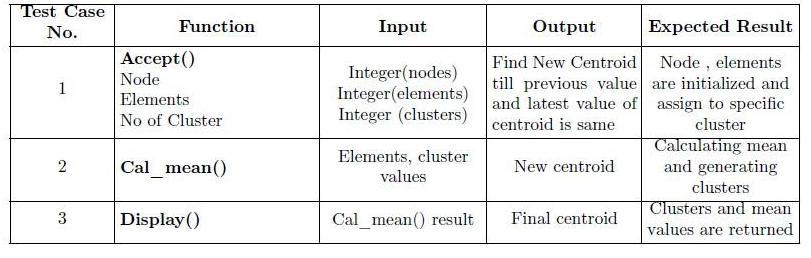
\includegraphics{204/Assignment_3(K-means)/temp.png}\\
	
	
	\noindent \textbf{ PSEUDOCODE: } \\ \\
	Pseudo code forcalmean() :static \\
	void calmean() \\
	{ \\
		int \\
		temp1=0;for(inti=0;i<p;++i) \\
		{
			if(a>m[i])dif[i]=am[i]; \\
			elsed if [i]=m[i]-a; \\
		} \\
		int val=0; \\
		double \\
		temp=dif[0];for(inti=0;i< p;++i) \\
		{ \\
			if(dif[i]<temp) \\
			{ \\
				temp=dif[i]; \\
				val=i; \\
		}} \\
		returnval; \\
	}\\
	
	\noindent \textbf{ CONCLUSION:}
	Thus, we have implemented K-means clustering algorithm using Java.
	
	\begin{center}
		\begin{tabular}{|c|c|c|c|c|}
			\hline
			
			{\bf Roll No.}		&{\bf Name of Student}	&{\bf Date of Performance}  				&{\bf Date of Submission}	&{\bf Sign.}  \\    \hline
			BECOC357	& Sunny Shah  & 31 / 08 / 2017		& 21 / 09 / 2017		&  \\ \hline
		\end{tabular}•
	\end{center}
	
\end{document}